\chapter{First order transition Hamiltonian}
First order transition Hamiltonian can be written in a form
\begin{equation}
    \HH=\J_3-\frac{\tilde\lambda(t)}{2j}\left(\J_1+\tilde\chi(\J_3+j\Id)\right)^2
    \label{eq:firstOrderTransitionHamiltonianOriginal}
\end{equation}
for $\J=(\J_1,\J_2,\J_3)$ angular momentum operator, $\tilde\chi\in\R$ and $\tilde\lambda(t)$ some real time dependent parameter. The aim is to diagonalize this Hamiltonian to find the spectrum. To make driving parameters less entwined, we will instead use the Hamiltonian
\begin{equation}
    \HH=\J_3+\lambda\hat V_1 +\chi \hat V_2+\chi^2 \hat V_3,
    \label{eq:firstOrderTransitionHamiltonian}
\end{equation}
for
\begin{align}
    \hat V_1 &=-\frac{1}{2j}\J_1^2\\
    \hat V_2 &= -\frac{1}{2j}\left[\J_1(\J_3+j\Id)+(\J_3+j\Id)\J_1\right]\\
    \hat V_3 &= -\frac{1}{2j}(\J_3+j\Id)^2
\end{align}



Using the eigenbasis $\{\ket{j,m}\}$ for $j$ angular momentum quantum number and $m$ its projection to the direction $\J_3$ and defining
\begin{equation}
    \J_\pm\coloneqq\frac{1}{2}(\J_1\pm i\J_2),
\end{equation}
we get matrix elements
\begin{align}
    \braket{j'm'|\J^2|jm} &= j(j+1)\delta_{j'j}\delta_{m'm}\\
    \braket{j'm'|\J_3|jm} &= m \delta_{j'j}\delta_{m'm}\\
    \braket{j'm'|\J_\pm|jm} &= \sqrt{(j\mp m)(j\pm m+1)}\delta_{j'j}\delta_{m'm\pm 1},
\end{align}
where $\delta_{a'b}$ is Kronecker delta. Using
\begin{align}
        \left(\J_1+\chi(\J_3+j)\right)^2 &= \textcolor{purple}{\J_1^2} +\chi^2 (\J_3^2+j^2\Id+2j\J_3)+\chi(\textcolor{blue}{\J_1}\J_3+\J_3\textcolor{blue}{\J_1})+2\chi j\textcolor{blue}{\J_1}\\
        \textcolor{purple}{\J_1^2}&= \frac{1}{4}(\J_++\J_-)^2= \frac{1}{4}(\J_+^2+\J_-^2+\textcolor{violet}{\J_+\J_-}+\textcolor{violet}{\J_-\J_+})\\ 
        \textcolor{violet}{\J_\pm\J_\mp}&=\J^2-\J_3^2 \mp \J_3\\
        \textcolor{blue}{\J_1}&=(\J_+ +\J_-),
\end{align}
we get pentadiagonal matrix representation of $\HH$.
% \begin{equation}
%     \HH=\begin{pmatrix}
%         h_a   &h_b   &h_c   &0     &\dots &0\\
%         h_b   &\ddots&\ddots&\ddots&\ddots&\vdots\\
%         h_c   &\ddots&\ddots&\ddots&\ddots&0\\
%         0     &\ddots&\ddots&\ddots&\ddots&h_c\\
%         \vdots&\ddots&\ddots&\ddots&\ddots&h_b\\
%         0     &\dots &0     &h_c   &h_b   &h_a\\
%     \end{pmatrix}
% \end{equation}


\section{Hamiltonian analysis}
The behavior of cases $N=1$ and $N=2$ is not characteristic for our Hamiltonian and has no physical meaning in this case, therefore the properties of $N=3$ case will be discussed at first and afterwards generalized to arbitrary $N$ along with the limit $N\rightarrow$. Due to complexity of chosen Hamiltonian, only some aspects are possible to calculate analytically, but mostly the numerical analysis is needed.



\subsection{Case N=3}
The lowest dimension with characteristics common to higher $N$ is 3 with Hamiltonian in eigenbasis
\begin{equation}
    \HH=\left(
        \begin{array}{cccc}
         -\frac{ \lambda +6}{4} & -\frac{\chi }{2 \sqrt{3}} & -\frac{\lambda }{2 \sqrt{3}} & 0 \\
         -\frac{\chi }{2 \sqrt{3}} & \frac{ \left(-7 \lambda -4 \chi ^2-6\right)}{12} & -\chi  & -\frac{\lambda }{2 \sqrt{3}} \\
         -\frac{\lambda }{2 \sqrt{3}} & -\chi  & \frac{ \left(-7 \lambda -16 \chi ^2+6\right)}{12} & -\frac{5 \chi }{2 \sqrt{3}} \\
         0 & -\frac{\lambda }{2 \sqrt{3}} & -\frac{5 \chi }{2 \sqrt{3}} & -\frac{\lambda }{4}-3 \chi ^2+\frac{3}{2} \\
        \end{array}
        \right).
\end{equation}
Spectrum of this Hamiltonian can be written in analytically using some substitutions $A,B,C,D$, see Appendix \ref{appendix1}, as
\begin{align}
        E_0 &= \frac{1}{12} \left(G-F-\frac{\sqrt{D-E}}{2}\right)
        \label{eq:N=3_en0}\\
        E_1 &= \frac{1}{12}  \left(G-F+\frac{\sqrt{D-E}}{2}\right)
        \label{eq:N=3_en1}\\
        E_2 &= \frac{1}{12} \left(G+F-\frac{\sqrt{D+E}}{2}\right)
        \label{eq:N=3_en2}\\
        E_3 &= \frac{1}{12}  \left(G+F+\frac{\sqrt{D+E}}{2}\right).
        \label{eq:N=3_en3}
\end{align}
Eigenvectors can also be written analytically, but due to their compexity its better to analize them only numerically. Sections $\lambda=1$ and $\chi=1$ are shown in figures \ref{fig:N=3_energiesl},\ref{fig:N=3_energiesc}
\begin{figure}[h]
    \centering
    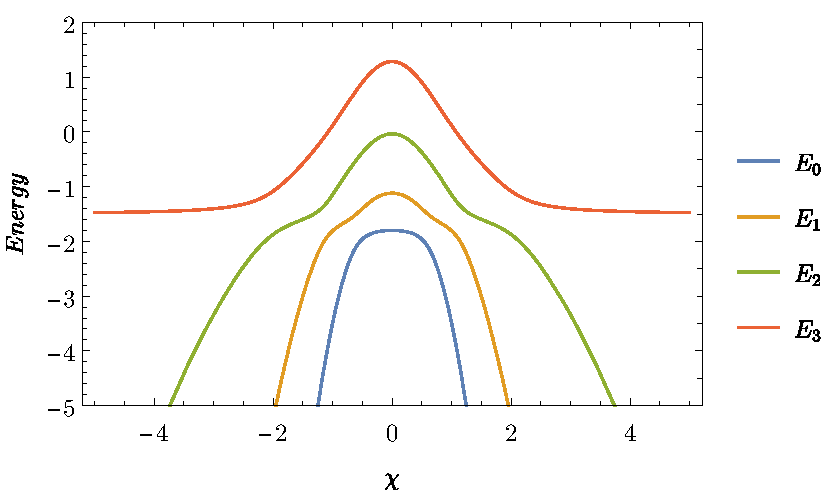
\includegraphics{../img/N=3_energiesl.pdf}
    \caption{Energy for the case $N=3$ Hamiltonian, section $\lambda=1$}
    \label{fig:N=3_energiesl}
\end{figure}
\begin{figure}[h]
    \centering
    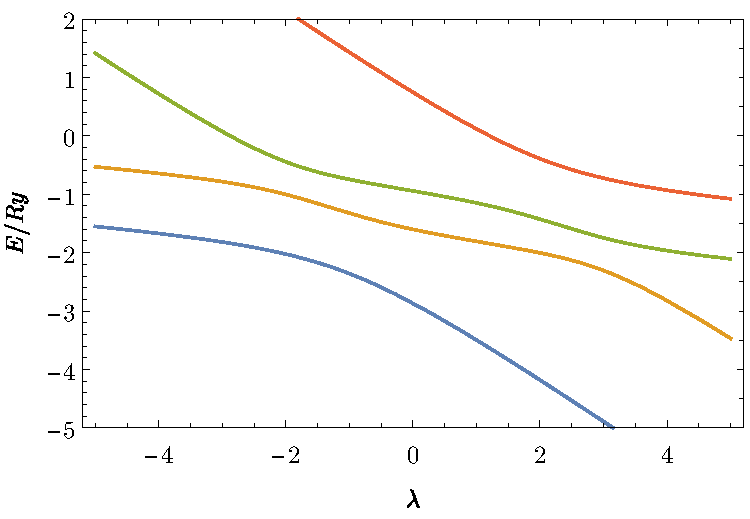
\includegraphics{../img/N=3_energiesc.pdf}
    \caption{Energy for the case $N=3$ Hamiltonian, section $\chi=1$}
    \label{fig:N=3_energiesc}
\end{figure}

From equations \ref{eq:N=3_en0}, \ref{eq:N=3_en1} can be seen that $E_0=E_1$ for $D=E$, which for real values $\lambda,\;\chi$ has two solutions
$$(\lambda_d,\pm \chi_d)=\left(-\frac{1}{2},\pm\sqrt{\frac{3}{5}}\right).$$
Point-like characteristics corresponds to Theorem \ref{thm:n-2}, which states that Hamiltonian driven by two real parameters can be degenerated only on 0-dimensional manifolds. 

If the energy spectrum is degenerate and metric tensor diverges, see individual elements on fig. \ref{fig:N=3_g}, its determinant also diverges, as shown on fig. \ref{fig:N=3_gDivenrgence}, along with Christoffel symbols elements, see fig. \ref{fig:N=3_G}. Note that metric tensor determinant is positive definite, thus the manifold is Riemannian. Further on it reflects symmetry $\chi\leftrightarrow-\chi$, except for off-diagonal elements, i.e. $g_{12}$, $\Gamma_{121}$, $\Gamma_{211}$, $\Gamma_{222}$, which switches their sign.
\begin{figure}
    \centering
    \begin{tabular}{cc}
    \subcaptionbox{$\arctan(g_{11})$}{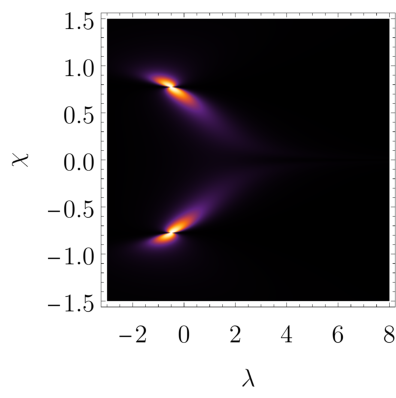
\includegraphics{../img/N=3_g11.pdf}} \\
    \subcaptionbox{$\arctan(g_{12})$}{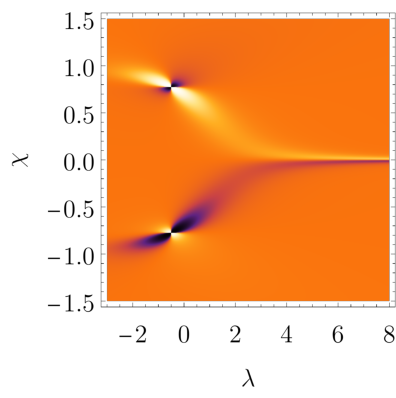
\includegraphics{../img/N=3_g12.pdf}}\\
    \subcaptionbox{$\arctan(g_{22})$}{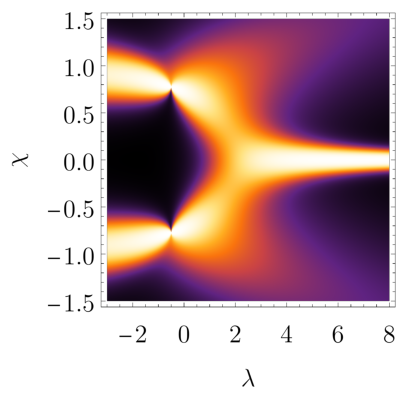
\includegraphics{../img/N=3_g22.pdf}}\\
    \end{tabular}
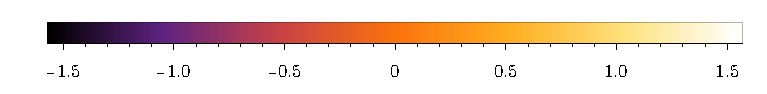
\includegraphics{../img/N=3_barA.pdf}
    \caption{Arcustangens of metric tensor elements for the case $N=3$}
    \label{fig:N=3_g}
\end{figure}

\begin{figure}[h]
    \centering
    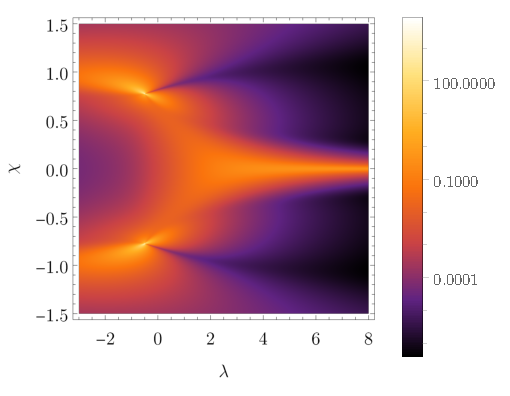
\includegraphics{../img/N=3_gDivergence.pdf}
    \caption{Metric determinant in a parameter space for $N=3$.}
    \label{fig:N=3_gDivenrgence}    
\end{figure}


\begin{figure}[h]
    \centering
    \begin{tabular}{cc}
    \subcaptionbox{$\arctan(\Gamma_{111})$}{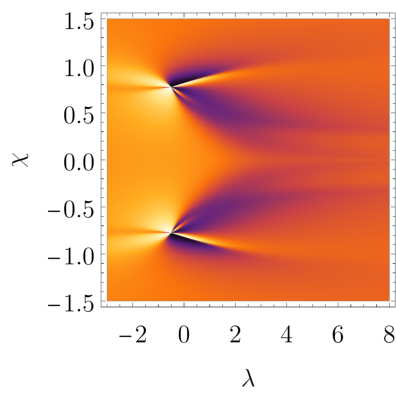
\includegraphics{../img/N=3_G111.pdf}} &
    \subcaptionbox{$\arctan(\Gamma_{211})$}{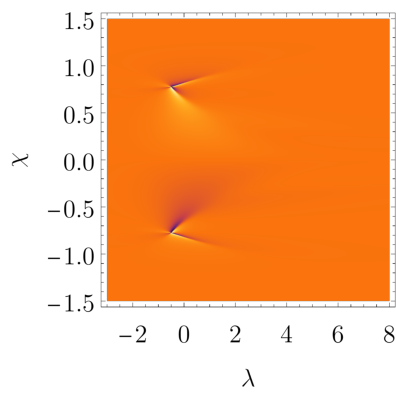
\includegraphics{../img/N=3_G211.pdf}} \\
    \subcaptionbox{$\arctan(\Gamma_{121})$}{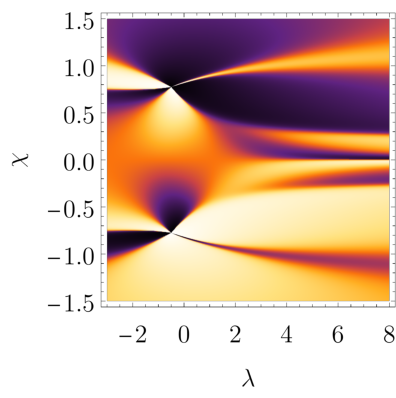
\includegraphics{../img/N=3_G121.pdf}} &
    \subcaptionbox{$\arctan(\Gamma_{221})$}{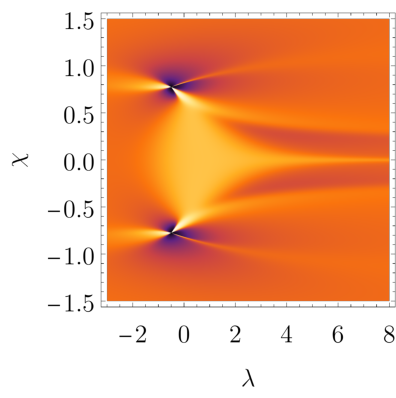
\includegraphics{../img/N=3_G221.pdf}}\\
    \subcaptionbox{$\arctan(\Gamma_{122})$}{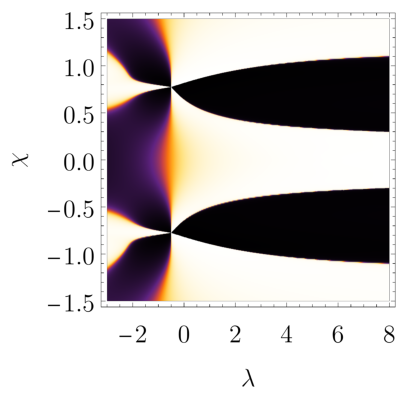
\includegraphics{../img/N=3_G122.pdf}} &
    \subcaptionbox{$\arctan(\Gamma_{222})$}{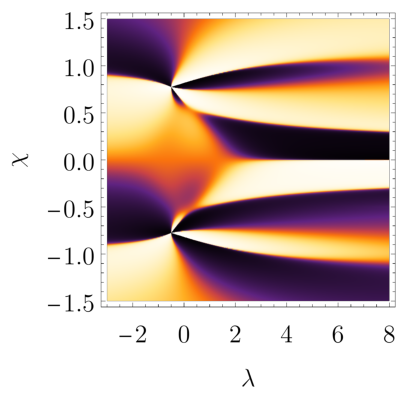
\includegraphics{../img/N=3_G222.pdf}}\\
    \end{tabular}
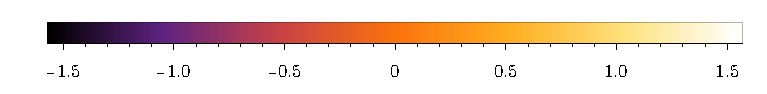
\includegraphics{../img/N=3_barA.pdf}
    \caption{Arcustangens of Christoffel symbols for the case $N=3$}
    \label{fig:N=3_G}
\end{figure}

Due to metric tensor degeneracy, the space is not geodesically complete and according to \ref{thm:hopf-Rinow_modified} there exist some "event horizon" around singularities $(\lambda_d,\pm \chi_d)$. This can be seen more clearly from geodesics, i.e. by solving initial value problem with conditions
$$(\lambda(t_i);\chi(t_i))=(\lambda_i;\chi_i)$$
$$\left(\der{\lambda(t)}{t};\der{\chi(t)}{t}\right)\Bigg|_{t_i}=(\lambda'_i;\chi'_i).$$

Results for these geodesics starting at $(\lambda;\chi)=(0;0), (\lambda',\chi')=(\cos\theta;\sin\theta)$ for $\theta\in [-0.63;0.63]$ and $\theta\in [\pi-0.225;\pi+0.225]$ with step $0.01$, see fig \ref{fig:N=3_geodesics}. Other values $\theta$ result in close approach of the geodesics to singularity making calculations numerically unstable. The fact that geodesics tend to lean towards singularities is well known from the theory of General Relativity (GR). The main difference here is, that our "test particle" seems to be partiallz repulsed from the singularity, see charge attraction vs. repulsion intuition in fig. \ref{fig:geodesicsinGR}. \textcolor{blue}{This is caused by the fact, that the Hamiltonian consists of more elements from which some are "repulsive" and some "attractive". }

\begin{figure}[h]
    \centering
    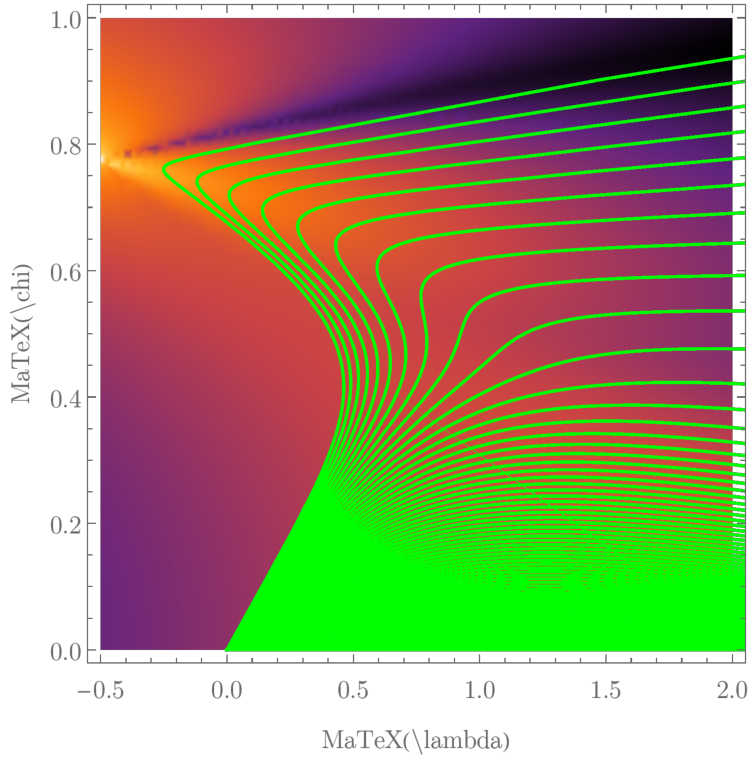
\includegraphics{../img/N=3_geodesics.pdf}
    \caption{Geodesics starting from $(\lambda_i;\chi_i)=(0;0)$ with $(\lambda'_i;\chi'_i)=(\cos\theta;\sin\theta)$ $N=3$.}
    \label{fig:N=3_geodesics}    
\end{figure}
\begin{figure}[h]
    \centering
    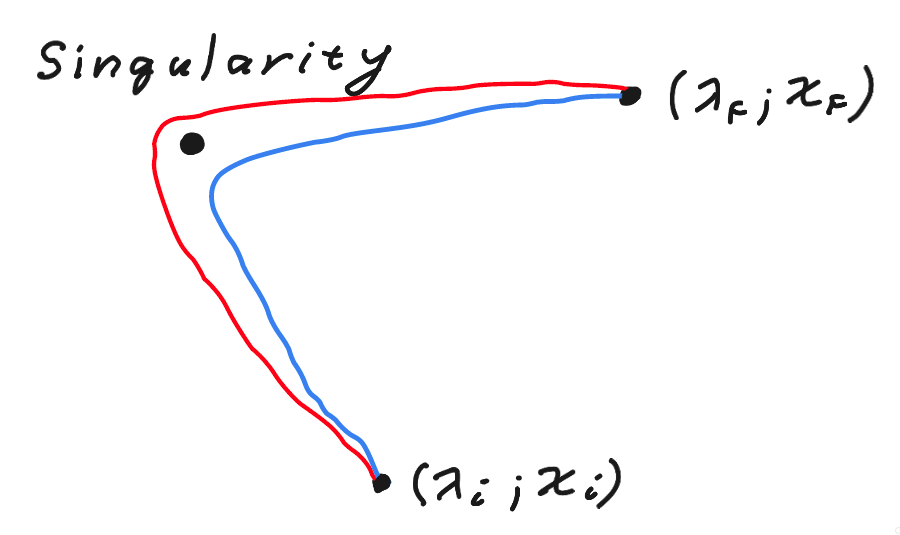
\includegraphics[width=0.6\textwidth]{../img/geodesicsinGR.png}
    \caption{Comparing geodesics with repulsing (blue) and attracting (red) metric tensor divergence in the spherical symmetrical space. }
    \label{fig:geodesicsinGR}
\end{figure}


\newpage
\section{Arbitrary $N$}
Looking at the energy spectrum of $N=10$ case (see section for $\lambda=1$ on fig. \ref{fig:N=10_energiesl} and section $\chi=1$ in fig. \ref{fig:N=10_energies2}) we see the characteristic structure of the system. Between every two energy levels is at least one avoided crossing. Another interesting aspect are metric tensor singularities, which are moving along \textcolor{blue}{line}, which was using linear regression from datapoints in fig. \ref{fig:singularitiesRegr} approximated as 
\begin{equation}
    \chi=-0.14 \lambda + 0.71
    \label{eq:linearRegressionSingularities}
\end{equation}
 


\begin{figure}[h]
    \centering
    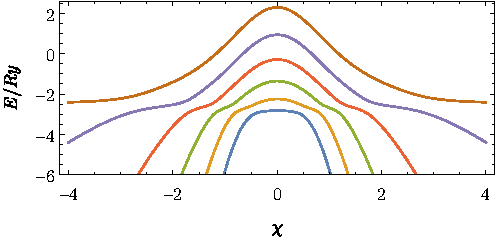
\includegraphics{../img/N=10_energiesl.pdf}
    \caption{Energy spectrum as function of $\chi$, for $\lambda=1$ and $N=10$.}
    \label{fig:N=10_energiesl}    
\end{figure}
\begin{figure}[h]
    \centering
    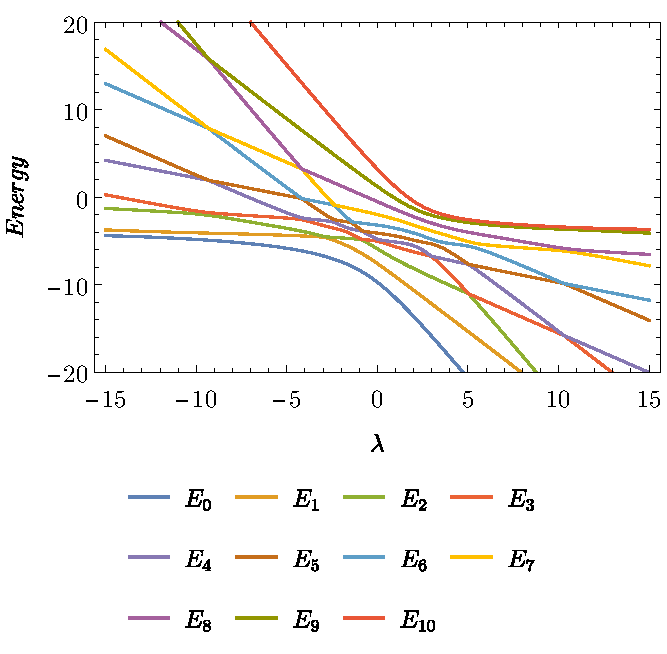
\includegraphics{../img/N=10_energies2.pdf}
    \caption{Energy spectrum as function of $\lambda$, for $\chi=1$ and $N=10$.}
    \label{fig:N=10_energies2}    
\end{figure}

\begin{figure}[h]
    \centering
    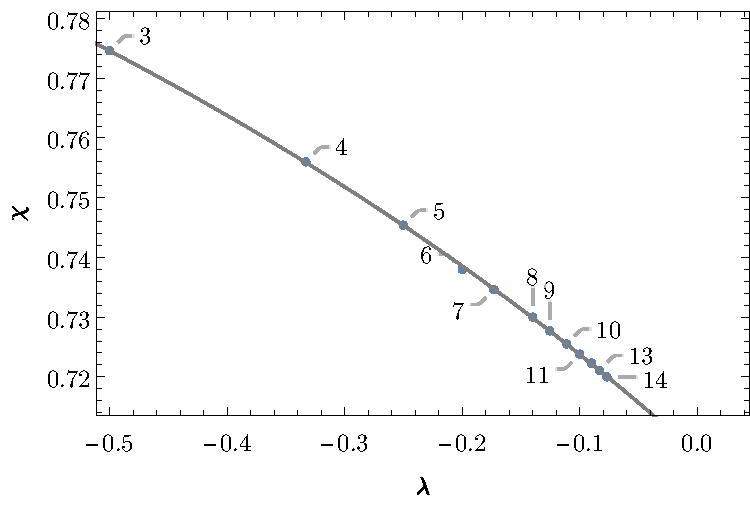
\includegraphics{../img/divPosition.pdf}
    \caption{Singularities in the metric tensor for different values of $N$ (see the numbers inside the plot) with linear regression according to eq. \ref{eq:linearRegressionSingularities}. Green points mark minimums.}
    \label{fig:singularitiesRegr}    
\end{figure}




\section{Limit $N\rightarrow \infty$}
In the limit $N\rightarrow \infty$, the first order transition lies in curve
\begin{equation}
    \chi^2=\frac{\lambda-1}{\lambda-2}
\end{equation}
and $\chi$-axis to the right from the point of second order transition, which lies in $(\lambda,\chi)=(1,0)$. On figure \ref{fig:transitionCompare} can be seen the transition curve with comparison to minimum between the ground state and first excited state for $N=3$ case. With increasing $N$, the line is slowly converging to the transition line.

\begin{figure}[h]
    \centering
    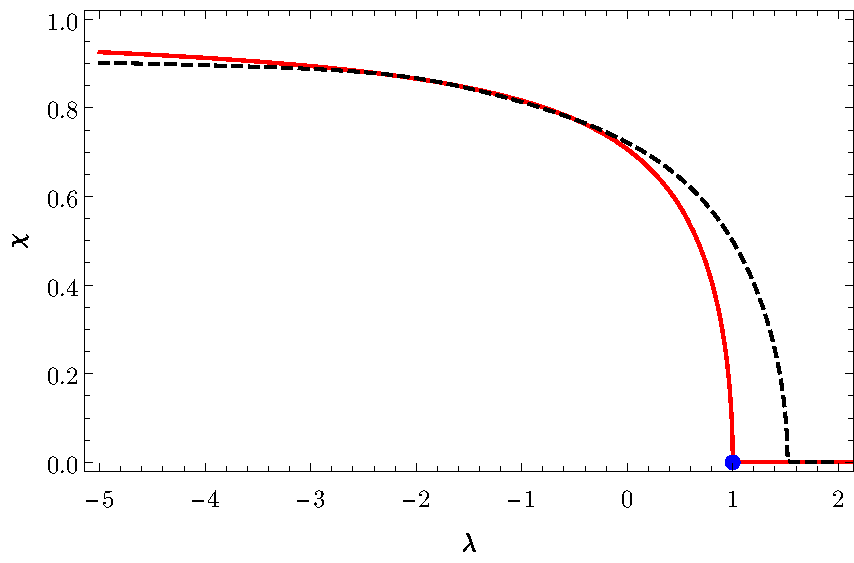
\includegraphics{../img/infiniteN_transitionCompare.pdf}
    \caption{First order transition (red), second order transition (blue point), minimum between the ground state and first excited state in N=3 case (black, dashed).}
    \label{fig:transitionCompare}    
\end{figure}